% Seção 5: Circuito de medição da temperatura interna

\section{Circuito de medição da temperatura interna}
\label{sec:pt100}

O circuito de condicionamento dos Pt100 é mostrado na Figura~\ref{fig:esq_pt100}.

\begin{figure}[H]
  \centering
  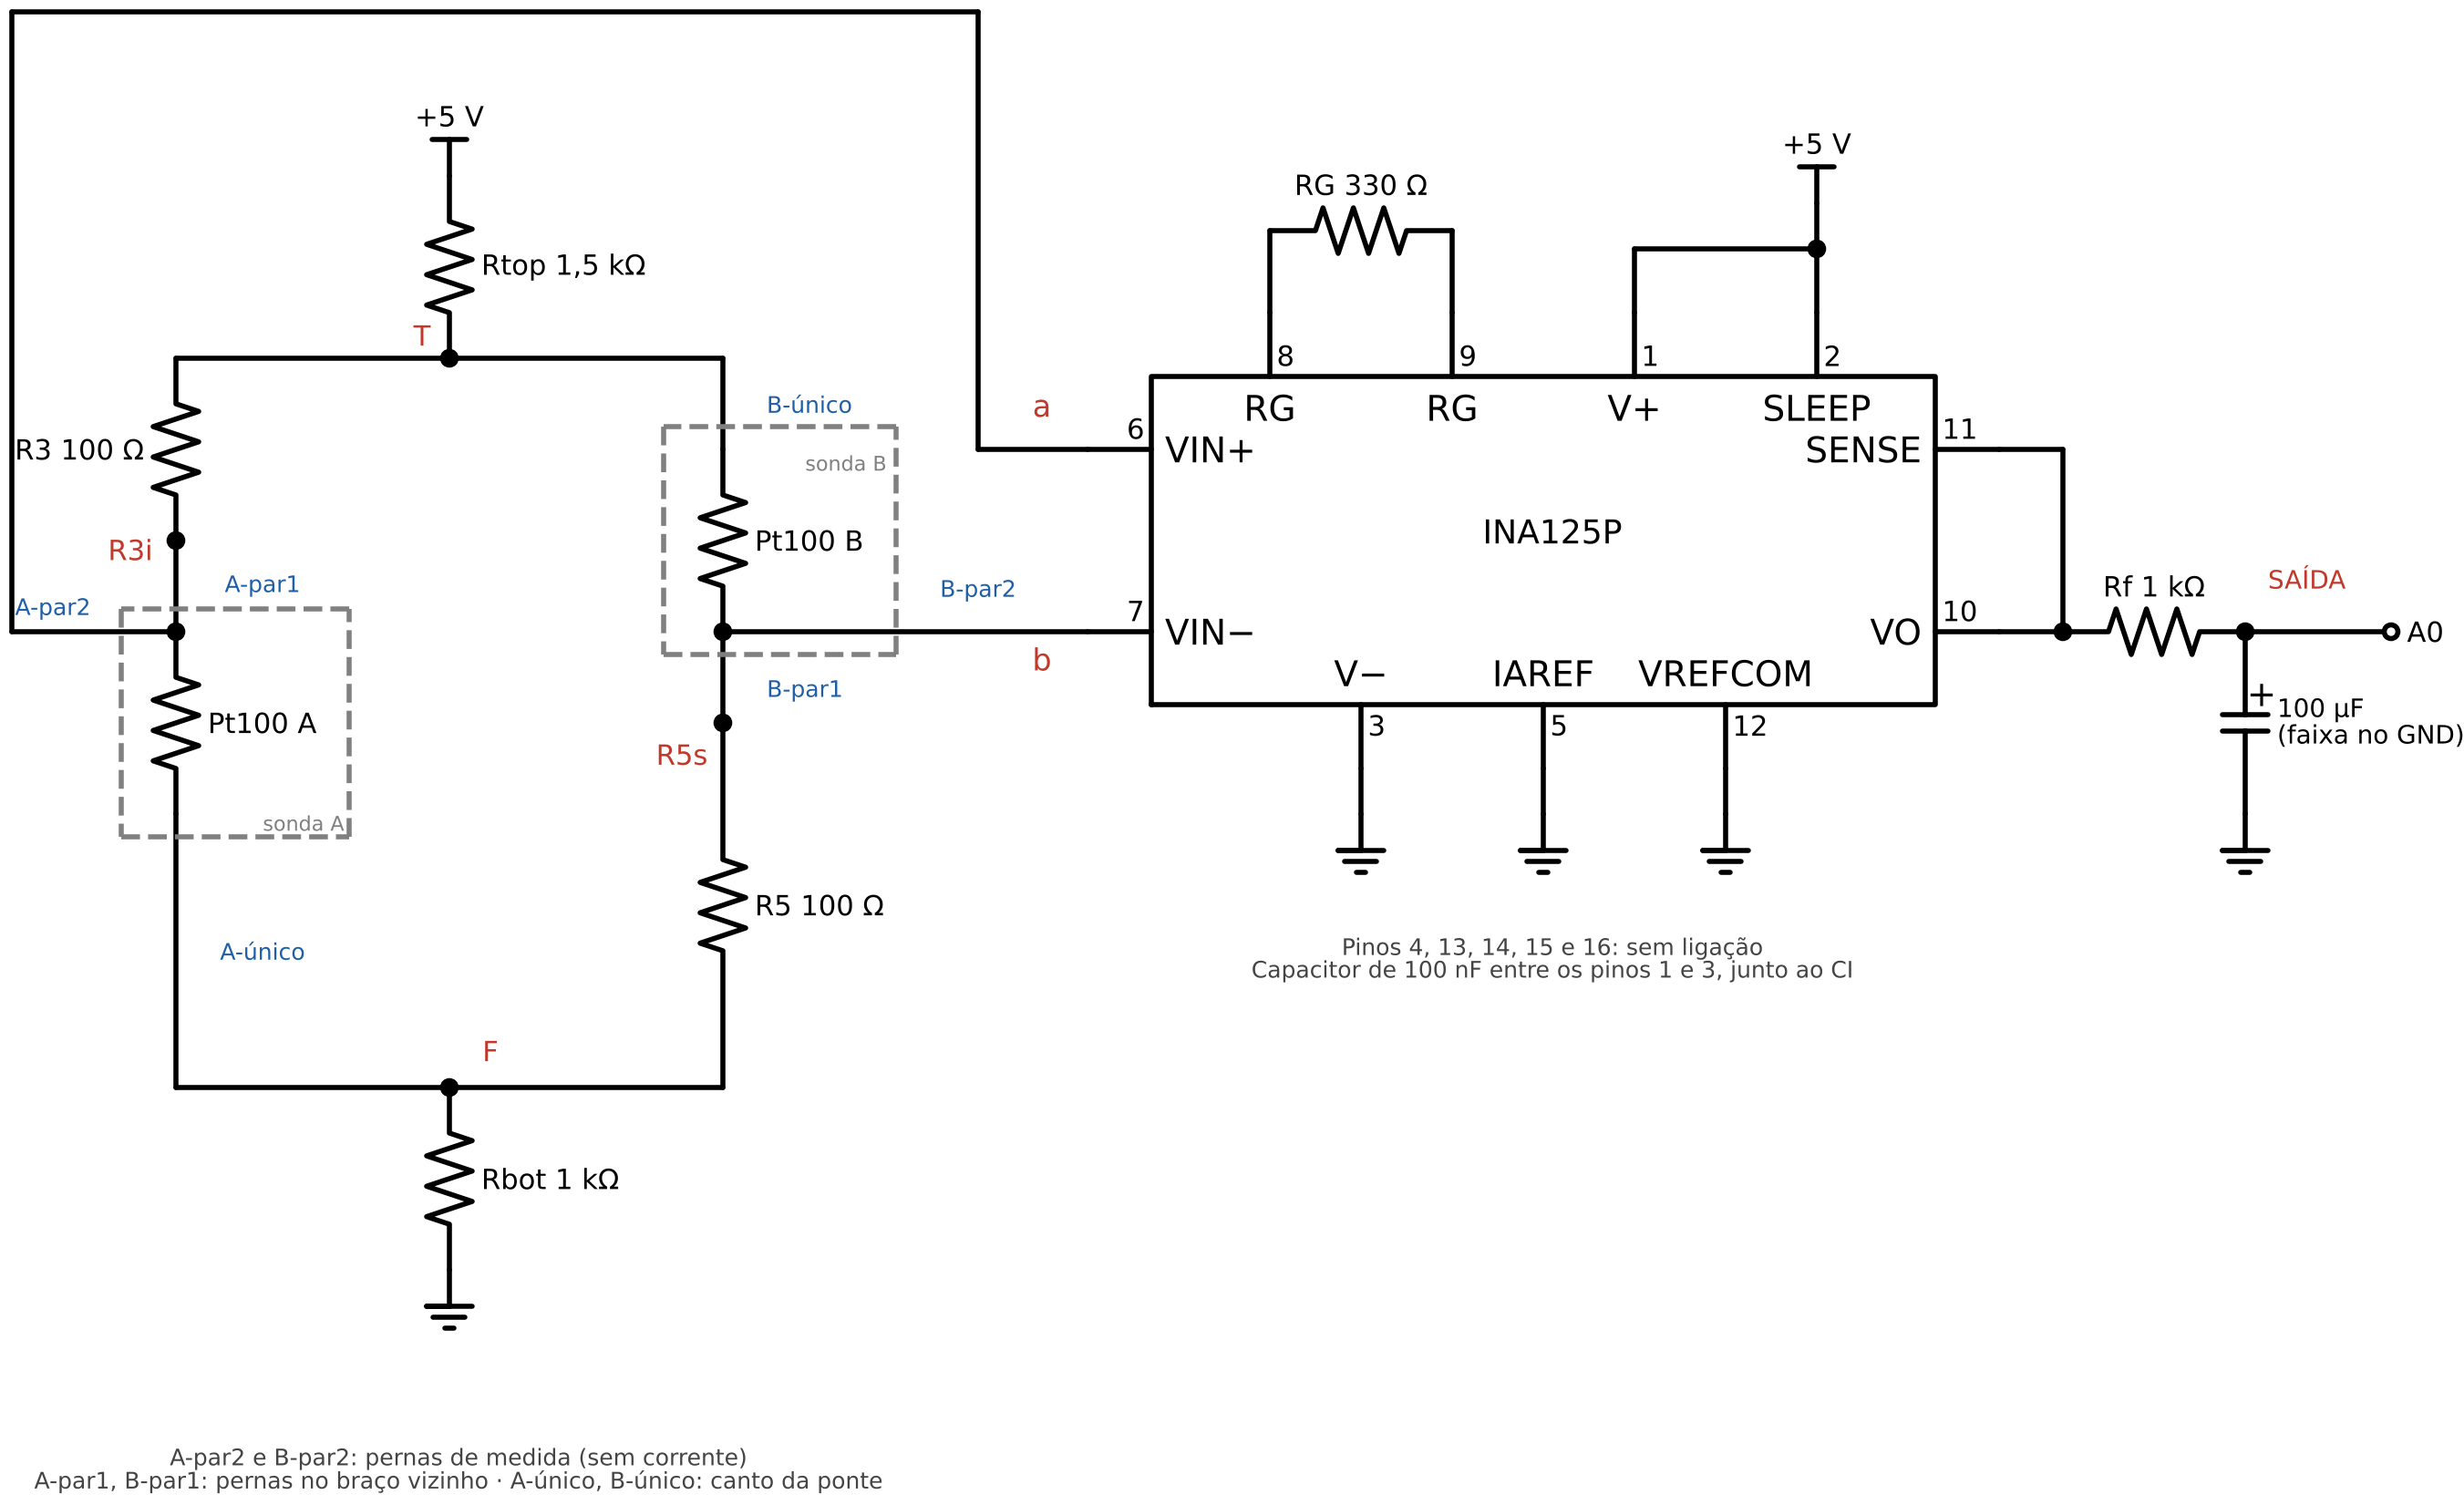
\includegraphics[width=\textwidth]{esq_pt100_ina125.png}
  \caption{Condicionamento dos Pt100: ponte de Wheatstone com dois sensores em braços opostos e ligação a 3 fios, amplificador de instrumentação INA125P e filtro anti-\textit{aliasing} na entrada A0.}
  \label{fig:esq_pt100}
\end{figure}

\paragraph{Ponte de Wheatstone.} Os dois Pt100 ficam em braços opostos da ponte, ambos dentro da câmara. Assim, quando a temperatura sobe, a tensão no nó $a$ aumenta e a do nó $b$ diminui, o que dobra a sensibilidade em relação a uma ponte com um único sensor. Os resistores de 100\,$\Omega$ equilibram a ponte em 0\,\ensuremath{^\circ}C.

\paragraph{Corrente nos sensores e modo comum.} Os resistores $R_{top}$ = 1,5\,k$\Omega$ e $R_{bot}$ = 1\,k$\Omega$ em série com a ponte limitam a corrente total a
\begin{equation}
  I = \frac{5}{1500 + 100 + 1000} \approx 1{,}92\ \text{mA},
\end{equation}
ou cerca de 0,96\,mA em cada Pt100. O autoaquecimento resultante ($I^2 R \approx 0{,}1$\,mW) é desprezível com a ventilação forçada. Esses resistores também posicionam as entradas do INA125P em aproximadamente 2,0\,V, dentro da faixa de modo comum do amplificador com alimentação única de 5\,V.

\paragraph{Sensibilidade e ganho.} Para pequenas variações de resistência, a saída da ponte é aproximadamente
\begin{equation}
  V_{ab} \approx I_{ramo}\,\Delta R = 0{,}96\ \text{mA} \times 0{,}385\ \Omega/{}^\circ\text{C} \approx 0{,}37\ \text{mV}/{}^\circ\text{C}.
\end{equation}
O ganho do INA125P é definido por $R_G$:
\begin{equation}
  G = 4 + \frac{60\ \text{k}\Omega}{R_G} = 4 + \frac{60\,000}{330} \approx 186,
\end{equation}
o que resulta em cerca de 69\,mV/\ensuremath{^\circ}C na saída e em uma resolução de aproximadamente 0,07\,\ensuremath{^\circ}C por LSB do conversor A/D. O pino SLEEP é ligado a V+, o pino SENSE à saída VO, e os pinos V$-$, IAREF e VREFCOM ao terra do Arduino. Os pinos da referência interna (4 e 13 a 16) não são utilizados.

\paragraph{Faixa de medição.} A saída do INA125P com alimentação única de 5\,V é considerada linear entre aproximadamente 0,8\,V e 4,2\,V. Com o ganho escolhido, isso corresponde à faixa de 12\,\ensuremath{^\circ}C a 61\,\ensuremath{^\circ}C, que cobre a faixa de operação prevista. Como a saída não ultrapassa a alimentação de 5\,V, a entrada do Arduino não precisa de diodos de proteção.

\paragraph{Ligação a 3 fios.} Cada Pt100 tem um par de fios ligado a uma das extremidades do sensor e um fio único ligado à outra. Em cada metade da ponte, a corrente percorre um fio do par, em série com o resistor de 100\,$\Omega$ do braço vizinho, e o fio único, em série com o próprio sensor. Como os dois braços de uma mesma metade recebem resistências de fio iguais, o efeito dos cabos se cancela com a ponte próxima do equilíbrio. O segundo fio do par leva a tensão do nó até a entrada do INA125P, que praticamente não drena corrente, de modo que a resistência desse fio não altera a medida.

\paragraph{Conversão e calibração.} Na faixa de 15\,\ensuremath{^\circ}C a 60\,\ensuremath{^\circ}C, o erro de não linearidade em relação a uma reta é de no máximo 0,11\,\ensuremath{^\circ}C (Seção~\ref{sec:simulacao}). A conversão de tensão em temperatura pode, portanto, ser linear. Como a tolerância de 1\,\% dos resistores da ponte gera um erro de offset de alguns graus, a reta será ajustada por calibração em dois pontos, comparando a leitura com um termômetro de referência.

\paragraph{Filtro.} O filtro RC na entrada A0, com $R_f$ = 1\,k$\Omega$ e $C_f$ = 100\,$\mu$F, tem constante de tempo de 0,1\,s e frequência de corte de
\begin{equation}
  f_c = \frac{1}{2\pi R_f C_f} \approx 1{,}6\ \text{Hz},
\end{equation}
muito acima da dinâmica térmica da câmara, que é da ordem de minutos. Ele atenua ruídos e o acoplamento do PWM. O resistor de 1\,k$\Omega$ também mantém baixa a impedância vista pelo conversor A/D.
